% ============================================================
% SECCIÓN: Tasas metabólicas y dinámica de crecimiento
% Desarrollo conceptual para tesis doctoral
% ============================================================

\section{Tasas metab\'{o}licas y din\'{a}mica de crecimiento}

Las tasas de flujo entre compartimentos constituyen el n\'{u}cleo operativo del modelo DEB. Cada tasa tiene unidades de masa de carbono por unidad de tiempo ($\si{mg\,C\,dia^{-1}}$) y representa un proceso fisiol\'{o}gico observable o inferible. En esta secci\'{o}n se derivan las expresiones matem\'{a}ticas de cada tasa, se explica su significado biol\'{o}gico y se discute el rol de los coeficientes log\'{i}sticos $\alpha$ y $\beta$ como perillas de calibraci\'{o}n del comportamiento fenot\'{i}pico.

\subsection{Tasa de asimilaci\'{o}n $r_A$}

La asimilaci\'{o}n es el proceso limitante global del metabolismo larval: todo el carbono que entra al sistema lo hace a trav\'{e}s de $r_A$. Eriksen la modela como proporcional a la biomasa estructural existente, con una tasa espec\'{i}fica $a$ que depende del \'{i}nstar:
\begin{equation}
    r_A = a\,B.
    \label{eq:rA}
\end{equation}

La tasa espec\'{i}fica $a$ se define por tramos (Figura~\ref{fig:tasas-alpha-beta}, panel inferior izquierdo):
\begin{equation}
    a =
    \begin{cases}
        a_{\max}, & I < 6, \\[6pt]
        a_{\max}\Bigl[1 - \bigl(\frac{B}{B_{\max}}\bigr)^{\alpha}\Bigr], & I = 6, \\[6pt]
        0, & I > 6 \;\text{(prepupa)}.
    \end{cases}
    \label{eq:a}
\end{equation}

\textbf{Interpretaci\'{o}n biol\'{o}gica.} Durante los instares 1--5 la larva se comporta como un sistema de crecimiento exponencial: su aparato digestivo est\'{a} subutilizado y puede procesar sustrato a la m\'{a}xima capacidad $a_{\max}$. Al entrar al instar 6, la larva alcanza una masa cr\'{i}tica cercana a $B_{\max}$ y activa mecanismos hormonales que reducen progresivamente la ingesta (m\'{o}dulo JH, ecdisona). El coeficiente $\alpha$ controla la \emph{forma} de esta reducci\'{o}n:
\begin{itemize}
    \item $\alpha = 1$: decaimiento log\'{i}stico puro (Verhulst), como en el modelo de \textcite{eriksenDynamicModellingFeed2022}.
    \item $\alpha < 1$: freno m\'{a}s brusco al inicio del instar 6; la larva ``se sacia'' antes.
    \item $\alpha > 1$: freno m\'{a}s suave; la larva sigue comiendo agresivamente hasta casi alcanzar $B_{\max}$.
\end{itemize}

En sustrato pollo est\'{a}ndar, Eriksen ajust\'o $\alpha = \num{0.92}$, es decir, un decaimiento ligeramente m\'{a}s pronunciado que el log\'{i}stico puro. Cuando el sustrato se diluye con lodo digerido (75\,\si{\percent}), $\alpha$ cae a $\num{0.28}$, indicando que la toxicidad o baja palatabilidad acelera el cese de la alimentaci\'{o}n \parencite{eriksenDynamicModellingFeed2022}.

\subsection{Mantenimiento $r_{\mathrm{CO_2},m}$}

El mantenimiento cubre todos los procesos energ\'{e}ticos que no generan s\'{i}ntesis neta: latido, osmorregulaci\'{o}n, movimiento, s\'{i}ntesis de ATP para homeostasis. Se modela como proporcional a la biomasa estructural, que representa la ``infraestructura'' que debe mantenerse:
\begin{equation}
    r_{\mathrm{CO_2},m} = m\,B.
    \label{eq:rCO2m}
\end{equation}

El par\'{a}metro $m = \SI{0.08}{\per\day}$ fue estimado por \textcite{laganaroGrowthMetabolicPerformance2021} a partir de respirometr\'{i}a en sustrato de pollo. Notablemente, $m$ no depende de $L$: los l\'{i}pidos de almacenamiento no requieren gasto energ\'{e}tico para mantener su integridad, a diferencia de los tejidos estructurales vivos.

\textbf{Conexi\'{o}n experimental.} En el reactor batch cerrado, $r_{\mathrm{CO_2},m}$ es la componente basal de la respiraci\'{o}n: incluso si la larva deja de crecer ($r_B = 0$) y de acumular grasa ($r_L = 0$), sigue emitiendo $m\,B$ de $\mathrm{CO_2}$. Esto explica por qu\'{e} el sensor NDIR nunca lee cero ppm entre ciclos de respirometr\'{i}a.

\subsection{Crecimiento estructural $r_B$ y la segunda log\'{i}stica $\beta$}

Si la asimilaci\'{o}n y el mantenimiento fueran los \'{u}nicos procesos, el crecimiento estructural seguir\'{i}a la tasa potencial:
\begin{equation}
    \mu_{B}^{\text{pot}} = \frac{a - m}{1 + Y_B},
    \label{eq:muB_pot}
\end{equation}
donde el denominador $1+Y_B$ refleja el costo energ\'{e}tico de convertir asimilados en biomasa: por cada $\si{mg\,C}$ de $B$ nuevo, se queman $Y_B = \num{0.44}\,\si{mg\,C}$ adicionales en $\mathrm{CO_2}$.

Sin embargo, \textcite{eriksenDynamicModellingFeed2022} observ\'{o} que las larvas de \textit{H.~illucens} acumulan l\'{i}pidos de forma creciente con la edad, lo cual no puede explicarse si $\mu_B^{\text{pot}}$ se consume enteramente en $r_B$. Introduce entonces una \textbf{segunda reducci\'{o}n log\'{i}stica}:
\begin{equation}
    \mu_B = \mu_{B}^{\text{pot}}\;\Bigl[1 - \Bigl(\frac{B}{B_{\max}}\Bigr)^{\beta}\Bigr] = \frac{a - m}{1 + Y_B}\;\Bigl[1 - \Bigl(\frac{B}{B_{\max}}\Bigr)^{\beta}\Bigr].
    \label{eq:muB}
\end{equation}

La tasa neta de s\'{i}ntesis de biomasa estructural es:
\begin{equation}
    r_B = \mu_B\,B \quad (I \le 6).
    \label{eq:rB}
\end{equation}

\textbf{El significado biol\'{o}gico de $\beta$.} Mientras $\alpha$ frena la \emph{entrada} de carbono (comer), $\beta$ frena la \emph{asignaci\'{o}n} de carbono a m\'{u}sculo y exoesqueleto (crecer). La diferencia entre lo que entra ($r_A$) y lo que se gasta en mantenimiento + crecimiento estructural genera un \textbf{excedente} que se canaliza hacia l\'{i}pidos. Por tanto:
\begin{itemize}
    \item $\beta$ alto ($> 2$): el crecimiento estructural se frena r\'{a}pido; la larva invierte tempranamente en grasa. Resultado: alto contenido lip\'{i}dico, peso final moderado.
    \item $\beta$ bajo ($< 1$): el crecimiento estructural persiste casi hasta $B_{\max}$; poco excedente para grasa. Resultado: larva grande y ``magra''.
\end{itemize}

En sustrato pollo, $\beta = \num{2.02}$ produce larvas con $\approx \SI{30}{\percent}$ de l\'{i}pidos al final del ciclo. En sustrato pobre, $\beta$ cae a $\num{0.90}$ y las larvas crecen m\'{a}s despacio, pero tambi\'{e}n m\'{a}s delgadas (Figura~\ref{fig:tasas-alpha-beta}).

\subsection{Acumulaci\'{o}n y reciclaje de l\'{i}pidos $r_L$}

El balance del pool de asimilados (Eq.~\ref{eq:dA_dt}) impone que el carbono sobrante tras cubrir mantenimiento y crecimiento vaya a l\'{i}pidos, o que los l\'{i}pidos se movilicen si falta carbono:
\begin{equation}
    r_L =
    \begin{cases}
        \dfrac{r_A - (r_B + r_{\mathrm{CO_2},m} + r_{\mathrm{CO_2},B})}{1 + Y_L}, & r_L \ge 0 \;\text{(acumulaci\'{o}n)}, \\[12pt]
        r_A - (r_B + r_{\mathrm{CO_2},m} + r_{\mathrm{CO_2},B}), & r_L < 0 \;\text{(reciclaje)}.
    \end{cases}
    \label{eq:rL}
\end{equation}

El costo de s\'{i}ntesis lip\'{i}dica $Y_L = \num{0.42}$ refleja la eficiencia de convertir carbohidratos en triacilgliceroles (ratio molar 72:168 de $\mathrm{CO_2}$:l\'{i}pido, seg\'{u}n \textcite{kok2021}). Cuando $r_L < 0$, los l\'{i}pidos se oxidan sin costo adicional ($r_{\mathrm{CO_2},L}=0$), ya que la hidr\'{o}lisis es energ\'{e}ticamente neutra o ligeramente exot\'{e}rmica.

\subsection{Emisi\'{o}n total de $\mathrm{CO_2}$}

La respiraci\'{o}n total es la suma de tres fuentes:
\begin{equation}
    r_{\mathrm{CO_2}} = \underbrace{m\,B}_{\text{mantenimiento}} + \underbrace{Y_B\,r_B}_{\text{costo crecimiento}} + \underbrace{Y_L\,r_L\,\mathbb{I}(r_L \ge 0)}_{\text{costo almacenamiento}},
    \label{eq:rCO2_total}
\end{equation}
donde $\mathbb{I}(\cdot)$ es la funci\'{o}n indicadora. La componente de mantenimiento domina al principio y al final del ciclo; la de crecimiento alcanza su m\'{a}ximo en el instar 6 temprano; la de l\'{i}pidos es menor pero sostenida, explicando la curva de $\mathrm{CO_2}$ acumulado en el batch cerrado.

\subsection{Determinaci\'{o}n del \'{i}nstar y biomasa m\'{a}xima din\'{a}mica}

El n\'{u}mero de \'{i}nstar no es una variable independiente sino una funci\'{o}n de $B$:
\begin{equation}
    I =
    \begin{cases}
        1\text{--}5, & B < \dfrac{1}{\delta_I}\,B_{\max,0}, \\[10pt]
        6, & \dfrac{1}{\delta_I}\,B_{\max,0} \le B < B_{\max,0}, \\[10pt]
        7\;\text{(prepupa)}, & B \ge B_{\max,0}.
    \end{cases}
    \label{eq:instar}
\end{equation}

Con $\delta_I = 5$, el umbral de muda del instar 5 al 6 ocurre en $B = 13\,\si{mg\,C}$. Esta regla es crucial porque activa la primera log\'{i}stica ($\alpha$) y desactiva eventualmente la alimentaci\'{o}n.

Finalmente, para capturar la variabilidad del peso final observada en cultivos reales (Fig.~2A de \textcite{eriksenDynamicModellingFeed2022}), $B_{\max}$ decrece linealmente tras un tiempo m\'{i}nimo de desarrollo $t_{p,\min} = \SI{13}{\day}$:
\begin{equation}
    B_{\max}(t) =
    \begin{cases}
        B_{\max,0}, & t < t_{p,\min}, \\[4pt]
        B_{\max,0} - \rho\,(t - t_{p,\min}), & t \ge t_{p,\min}.
    \end{cases}
    \label{eq:Bmax_t}
\end{equation}

El par\'{a}metro $\rho = \SI{1}{\milli\gram\,C\,\per\day}$ penaliza el retraso en la pupaci\'{o}n: larvas que tardan m\'{a}s de 13 d\'{i}as en alcanzar la prepupa sufren una reducci\'{o}n progresiva de su peso m\'{a}ximo te\'{o}rico. Esta funci\'{o}n, aunque lineal y emp\'{i}rica, reproduce la correlaci\'{o}n negativa entre tiempo de desarrollo y peso final reportada en la literatura \parencite{eriksenDynamicModellingFeed2022}.

\begin{figure}[htbp]
    \centering
    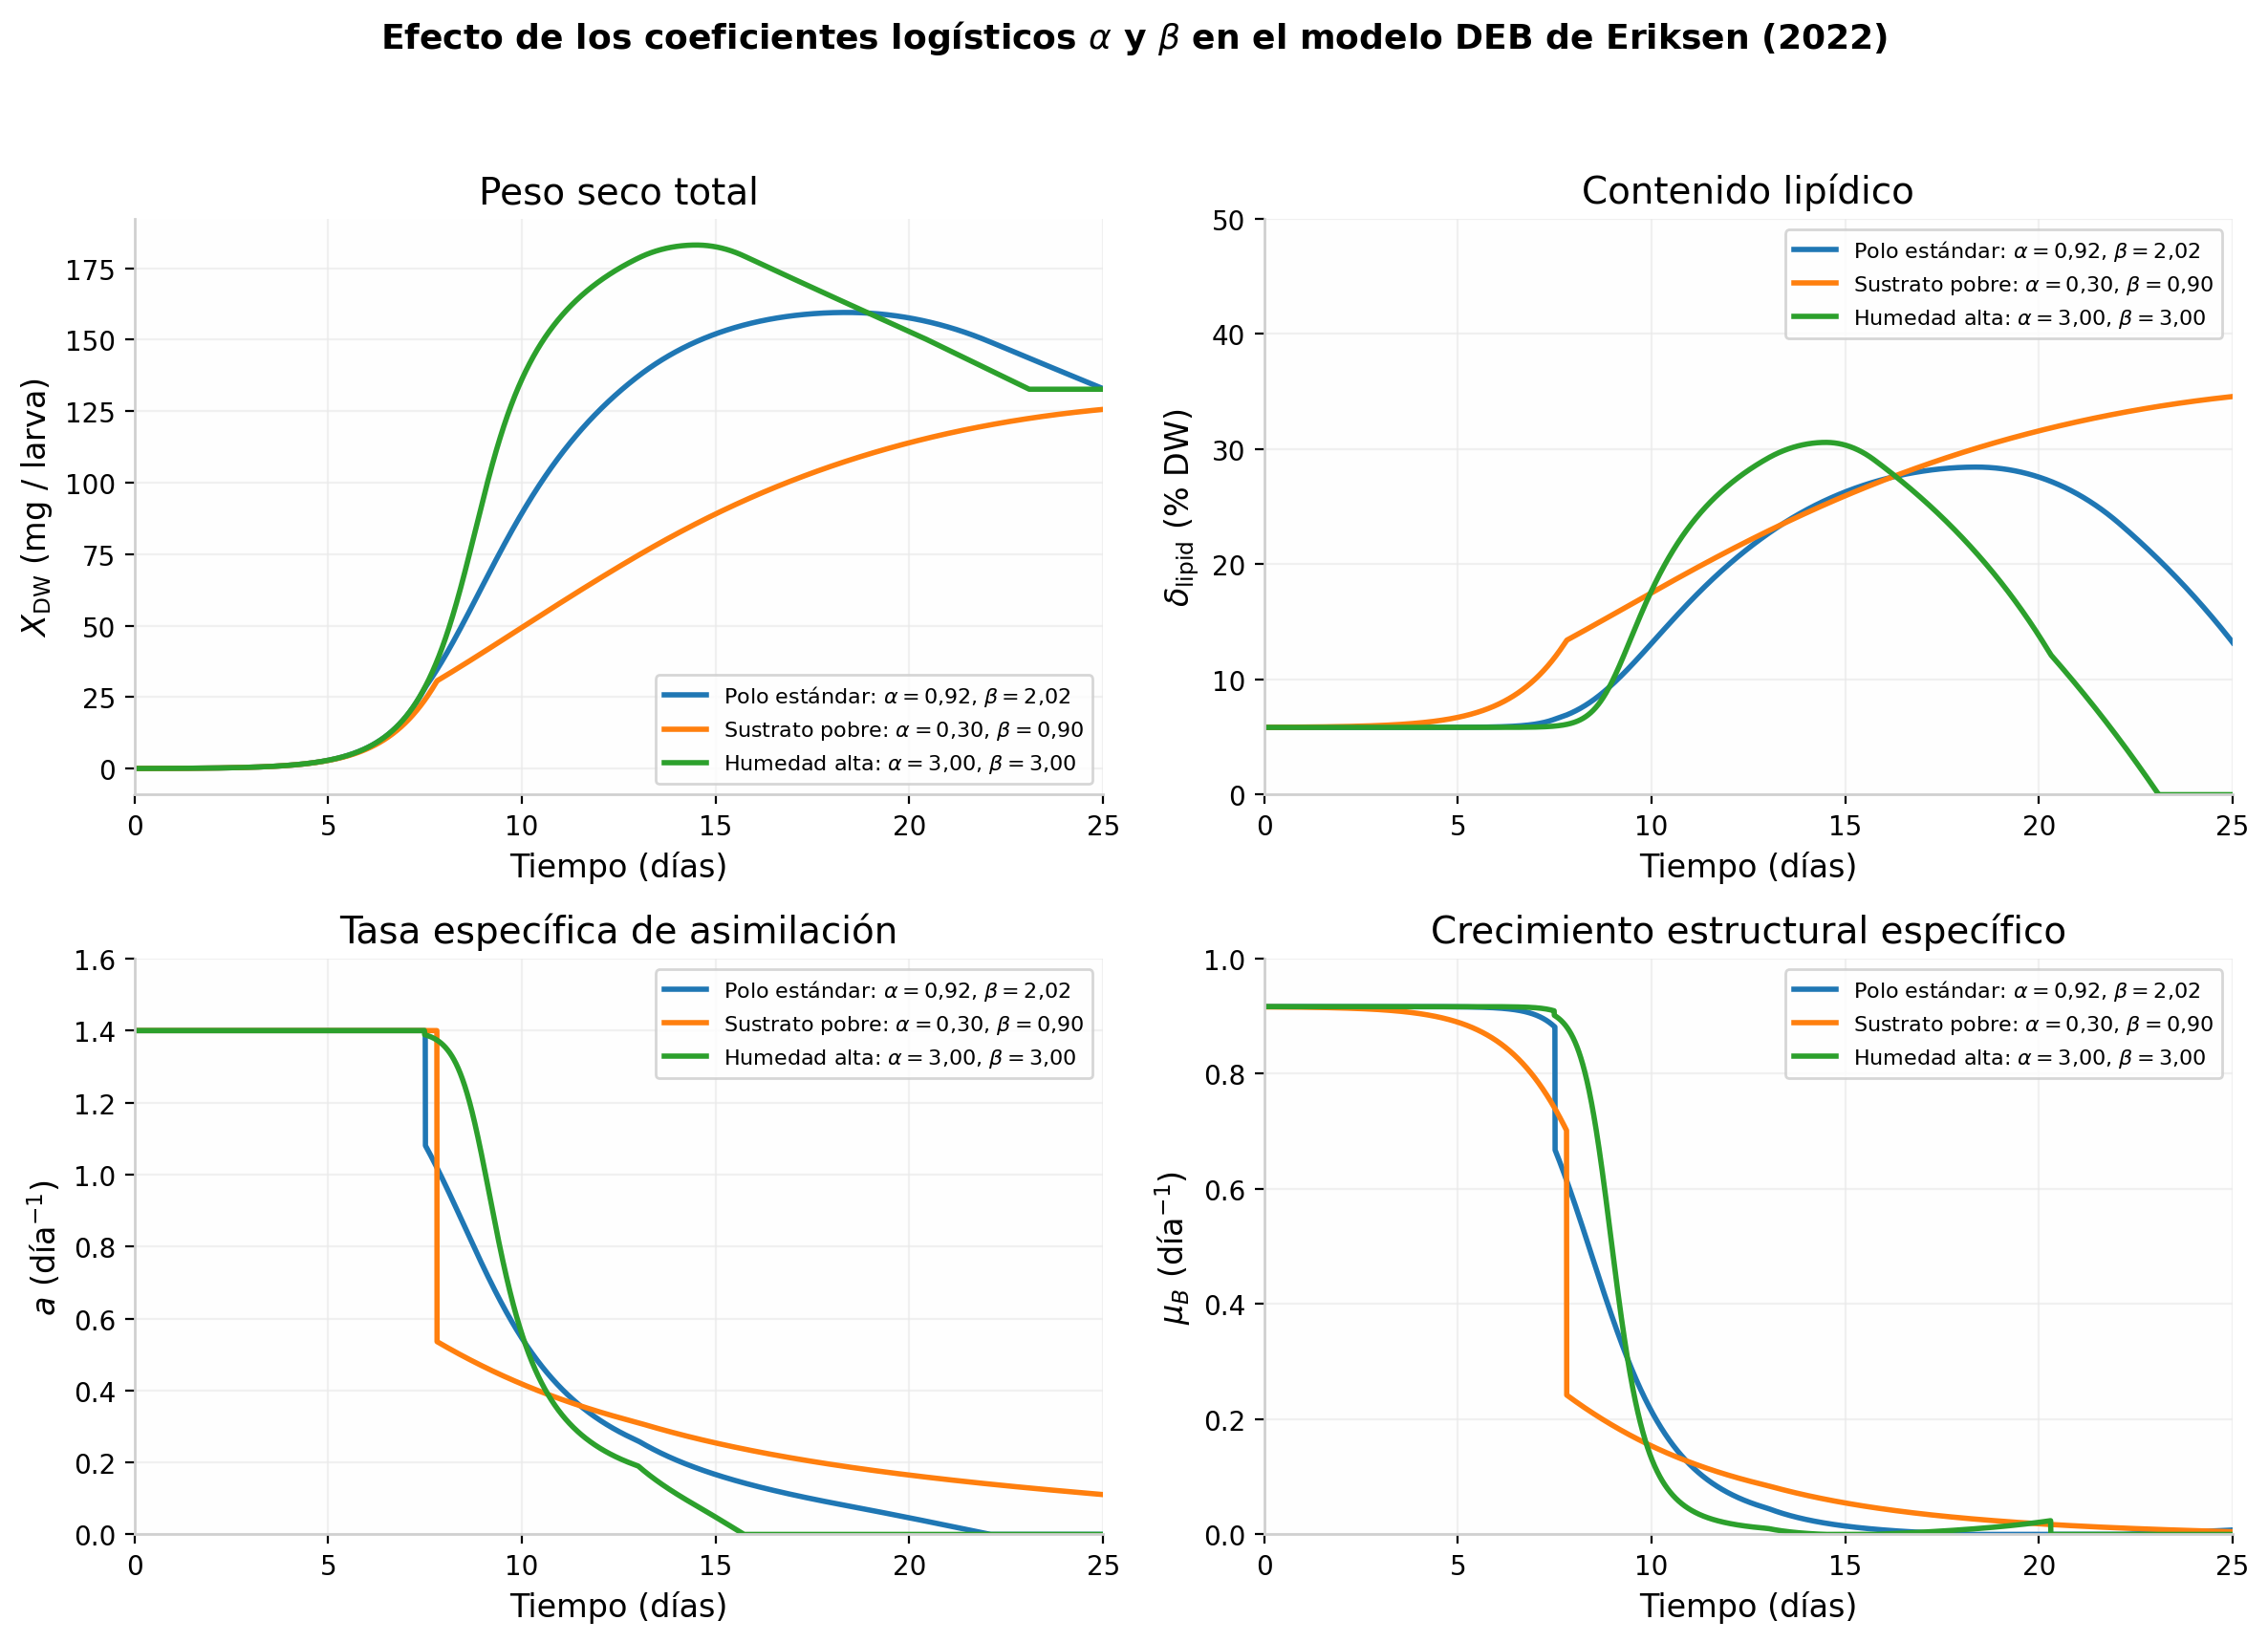
\includegraphics[width=0.95\textwidth]{00Figuras/fig_tasas_alpha_beta}
    \caption{Efecto de los coeficientes log\'{i}sticos $\alpha$ y $\beta$ en la din\'{a}mica del modelo DEB. Escenarios: (i) sustrato pollo est\'{a}ndar ($\alpha=0{,}92$, $\beta=2{,}02$); (ii) sustrato pobre con lodo digerido ($\alpha=0{,}30$, $\beta=0{,}90$); (iii) alta humedad ($\alpha=3{,}00$, $\beta=3{,}00$). Paneles superiores: peso seco total y contenido lip\'{i}dico. Paneles inferiores: tasas espec\'{i}ficas de asimilaci\'{o}n $a$ y crecimiento estructural $\mu_B$.}
    \label{fig:tasas-alpha-beta}
\end{figure}
